
\section{Dataset Preparation}
% \subsection*{Data Preprocessing}
% \subsection*{Prompt Preparation}

The Figure \ref{fig:prompt_pipeline} illustrates the overall pipeline of prompt preparation for GAN. This includes creating point prompts, bounding box prompts, and noisy mask prompts for the input adapter in phase 1 as well as creating prompts from auxiliary masks from automatic prompt generator from phase 3.

\begin{figure}[!h]
    \centering
    % 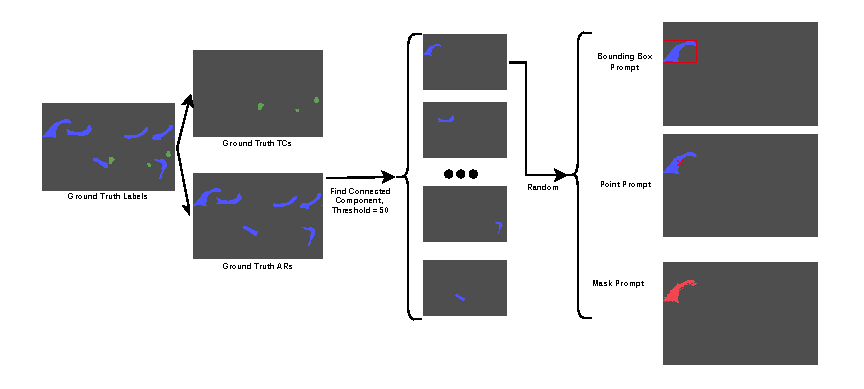
\includegraphics[width=1\textwidth]{graphics/approach/prompt_pipeline-1.pdf}
    \makebox[\textwidth][c]{%
    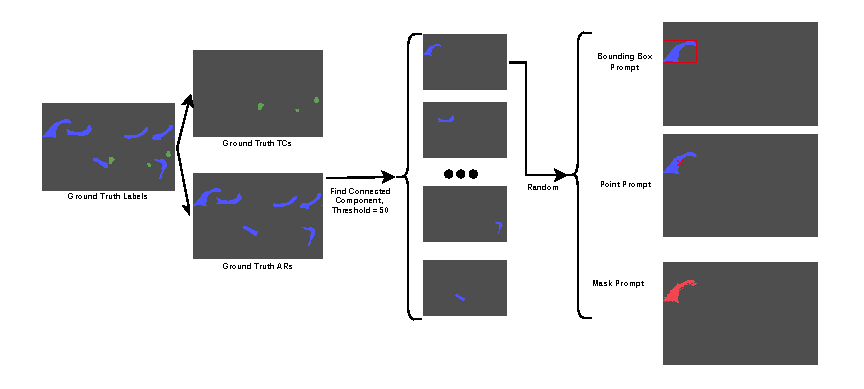
\includegraphics[width=1.2\textwidth]{graphics/approach/prompt_pipeline-1.pdf}
}
    \caption{Prompt Preparation Process}
    \label{fig:prompt_pipeline}
\end{figure}

The Figure \ref{fig:point_prompt_generation} and \ref{fig:noisy_mask_generation} describe the process of creating point prompts and noisy mask prompts in detail. To generate positive point prompts, the binary mask is first processed using an erosion operation with a kernel size determined by the object area. Positive points are then randomly sampled from this eroded region, ensuring the points remain well within the object boundaries. For negative point prompts, the pipeline utilizes two different dilation kernels. A smaller kernel and a big kernel are applied to the mask, and the smaller dilated version is subtracted from the larger one to define a boundary region for sampling negative points. 

\vspace{-2em}
\begin{figure}[!h]
    \centering
    % 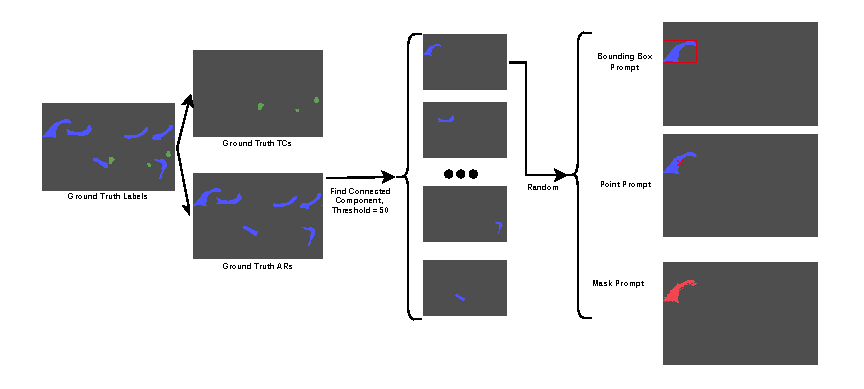
\includegraphics[width=1\textwidth]{graphics/approach/prompt_pipeline-1.pdf}
    \makebox[\textwidth][c]{%
    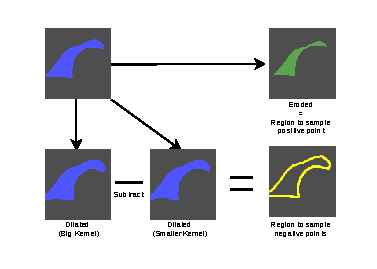
\includegraphics[width=0.7\textwidth]{graphics/approach/point_prompt.pdf}
}
\vspace{-2em}
    \caption{Sampling Negative and Positive Point Prompts}
    \label{fig:point_prompt_generation}
\end{figure}

The noisy mask prompt generation involves a multi-step interpolation and residue calculation process. The input mask is interpolated to a small size and then interpolated back to its original size to create a recovered mask. This recovered version is subtracted from the original input to identify incoherent regions. These regions are thresholded and then combined with Gaussian noise via element\_wise multiplication. Finally, the noise is integrated back into the mask through element\_wise addition to produce a dense, noisy mask prompt.

\vspace{-2em}
\begin{figure}[!h]
    \centering
    % 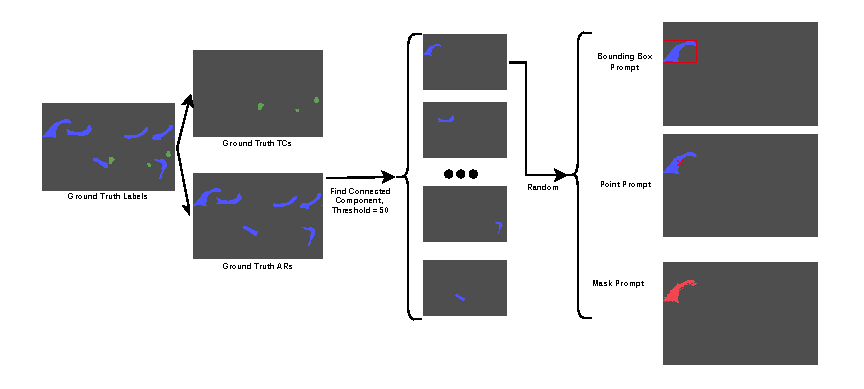
\includegraphics[width=1\textwidth]{graphics/approach/prompt_pipeline-1.pdf}
    \makebox[\textwidth][c]{%
    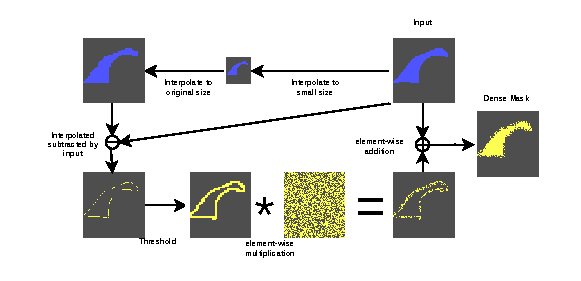
\includegraphics[width=1.2\textwidth]{graphics/approach/noisy_mask.pdf}
}
\vspace{-2em}
    \caption{Create Noisy Mask Prompts}
    \label{fig:noisy_mask_generation}
\end{figure}


% \begin{figure}[!h]
% \centering
% \vspace{-3em} 
% % Top Image
% % \begin{center}
% %     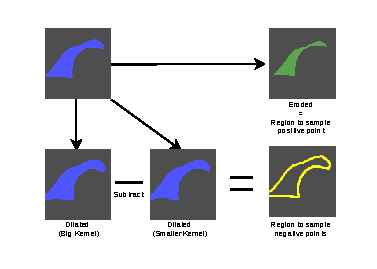
\includegraphics[width=0.7\textwidth]{graphics/approach/point_prompt.pdf}
% %     \caption{Sampling Negative and Positive Point Prompts}
% %     \label{fig:point_prompt_generation}
% % \end{center}
% \vspace{-3em} % Adds a small vertical gap between the two plots
% % Bottom Image
% \begin{center}
%     % \makebox[\textwidth][c]{%
%     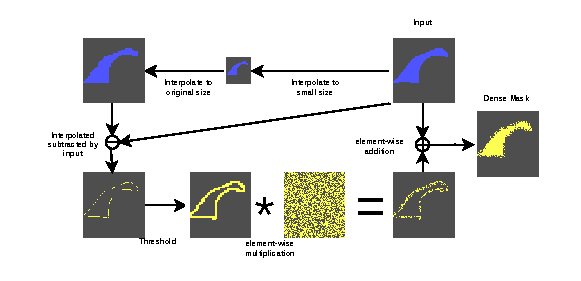
\includegraphics[width=1\textwidth]{graphics/approach/noisy_mask.pdf}
%     \caption{Create Noisy Mask Prompts}
%     \label{fig:noisy_mask_generation}
% \end{center}

% \caption{Prompt Generating Process}


% \end{figure}